% ----------------------- TODO ---------------------------
% Diese Daten müssen pro Blatt angepasst werden:
\newcommand{\NUMBER}{4}
\newcommand{\EXERCISES}{5}
% Diese Daten müssen einmalig pro Vorlesung angepasst werden:
\newcommand{\COURSE}{Grundlagen der Digitaltechnik}
\newcommand{\TOPIC}{Finite State Machines}
\newcommand{\DATE}{06.05.2022}
% ----------------------- TODO ---------------------------

\documentclass[a4paper]{scrartcl}

\usepackage[utf8]{inputenc}
\usepackage[ngerman]{babel}
\usepackage{amsmath}
\usepackage{amssymb}
\usepackage{fancyhdr}
\usepackage{color}
\usepackage{graphicx}
\usepackage{lastpage}
\usepackage{listings}
\usepackage{tikz}
\usepackage{pdflscape}
\usepackage{subfigure}
\usepackage{float}
\usepackage{polynom}
\usepackage{hyperref}
\usepackage{tabularx}
\usepackage{forloop}
\usepackage{geometry}
\usepackage{listings}
\usepackage{fancybox}
\usepackage{tikz}
\usepackage{algpseudocode,algorithm,algorithmicx}

%Definiere Let-Command für algorithmen
\newcommand*\Let[2]{\State #1 $\gets$ #2}

\input kvmacros

%Größe der Ränder setzen
\geometry{a4paper,left=3cm, right=3cm, top=3cm, bottom=3cm}

%Kopf- und Fußzeile
\pagestyle {fancy}
\fancyhead[L]{\COURSE}
\fancyhead[R]{\DATE}

\fancyfoot[L]{}
\fancyfoot[C]{}
\fancyfoot[R]{Seite \thepage /\pageref*{LastPage}}
\setlength{\parindent}{0pt}

%Formatierung der Überschrift, hier nichts ändern
\def\header#1#2{
  \begin{center}
    {\Large Labor #1: \TOPIC}\\
    {(Datum #2)}
  \end{center}
}


\begin{document}


\header{Nr. \NUMBER}{\DATE}

\section*{Aufgabe 1: Messablaufsteuerung}
Der Messablauf eines Spektrum Analyzers soll als Finite State Machine modelliert werden.
Der Messablauf hat folgende Zustände:
\begin{itemize}
  \item \textbf{Idle:} Es ist nichts zu tun.
  \item \textbf{Set HW:} Die Hardware wird für die nächste Messung richtig eingestellt.
  \item \textbf{Measurement:} Die Messung läuft.
  \item \textbf{Data Transfer:} Die gemessenen Daten werden in den User-RAM übertragen. 
  \item \textbf{Data Processing \& Presentation:} Die Daten im RAM werden prozessiert und zur Anzeige gebracht.  
\end{itemize}

Der Messablauf des Spektrum Analyzers ist grundsätzlich so:\\
Das \textbf{Start-Event} signalisiert den Start einer komplett neuen Messung. Dies führt zu dem Zustand \textbf{Set HW}. Der  \textbf{HW-Ready} Interrupt,
welcher direkt von der HW kommt, signalisiert dass die HW eingestellt ist und in den Zustand   \textbf{Measurement} gewechselt werden kann.
Wenn eine Messung beendet wurde, schickt die HW den Interrupt \textbf{Capturing Finished}, welcher zu einem Übergang in den Zustand \textbf{Data Transfer} führt.
Hier werden die Messdaten aus einem lokalen Buffer in der HW in den RAM des Host-PCs übertragen. Die Software meldet mit dem SW-Interrupt \textbf{Transfer Done},
dass 
alle Daten übertragen wurden. Dies führt zu einem Übergang in den Zustand \textbf{Data Processing \& Presentation}, welcher die transferierten
Daten zu einem ``Graphen'' aufbereitet und auf dem Display anzeigt. Dieser Schritt meldet sich fertig, in dem der SW-Interrupt \textbf{Data Displayed} 
gesetzt wurde.\\

Der Spektrum Analyzer kann in zwei Betriebsmodi betrieben werden: Continuous Mode und Single Shot Mode. Ist eine Messung im Continuous Mode fertig, soll
direkt mit einer neuen begonnen werden. Nach einer Messung im Single Shot Mode soll hingegen in den \textbf{Idle} Zustand gewechselt werden.\\

Das \textbf{Start-Event} wird von einer Taste am Messgerät erzeugt. Zusätzlich gibt es eine weitere Taste am Messgerät, welches ein \textbf{Abort-Event} schickt. Dieses
führt dazu, dass egal in welchem Zustand das Gerät sich gerade befindet, in den \textbf{Idle} Zustand gewechselt wird.


\subsection*{a) Zustandsgraphen}
Modelliere aus dem obigen Text einen Zustandsgraphen für das Messgerät. Schreibe in die ``Zustände'' den Namen, sowie die Codierungsnummer des Zustands 
(vgl. Slide: Entwurf von FSMs, Kapitel 6). Schreibe an die Pfeile (Transitionen) die Übergangsbedingung z.B. \textbf{Start-Event}.

\subsection*{b) Entwurf eines Mealy Automaten}
In der Vorlesung haben wir in Aufgabe 14 einen Mealy Automaten entworfen (s. Bild).
\begin{figure}[h!]
  \centering
  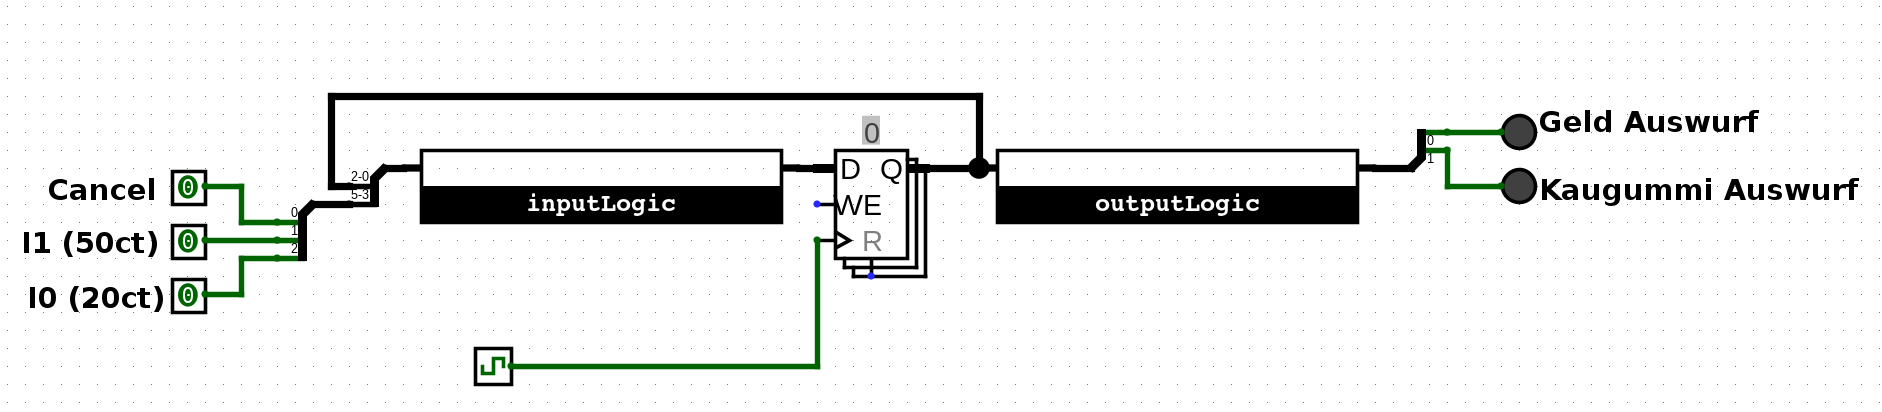
\includegraphics[width=\textwidth]{mealy.png}
\end{figure}

Dieser besteht aus einer Input-Logik, einem State-Register und einer Output-Logik. Mit dieser Vorlage soll nun für dieses Problem ein Mealy-Automat entworfen werden.

\subsubsection*{i) State-Register}
Es wird ein Register benötigt, welches alle möglichen Zustände des Messgeräts speichern kann.
\begin{enumerate}
  \item Ermittle die Anzahl an Zuständen
  \item Wähle ein ausreichend großes Register
\end{enumerate}


\subsubsection*{ii) Input-Logik}
Lege ein Subcircuit mit dem Namen ``Input-Logik'' an. Entwirf diesen nach den Infos aus dem Text.\\

\textbf{Hinweise:}
\begin{itemize}
  \item Die Eingänge für die Input-Logik sind alle im Text genannten Events (Interrupts), der Modus (single o. cont.), sowie der aktuelle Zustand.
  \item Der Ausgang der Input-Logik ist der neue Zustand
  \item Gehe von dem ``Schön Wetter Fall'' aus, das niemals zwei Eingangsevents gleichzeitig auftreten können (das Modesignal ist kein ``Event'')
  \item Auch der Cont. und Single-Shot Mode können nicht gleichzeitig auftreten, während einer Messung ist aber immer einer der beiden aktiv
  \item Eine Möglichkeit wäre durch die Events eine Auswahlschaltung zu erstellen und für jedes Event eine ``eigene Eventlogik'' zu erstellen (divide \& conquer)
  \item Die Tabellen am Ende des Dokuments können beim Erstellen der Logik helfen 
\end{itemize}


\subsubsection*{iii) Output-Logik}
Lege ein Subcircuit mit dem Namen ``Output-Logik'' an. Eigentlich müsste die Output-Logik der 
FSM jetzt aus den Zuständen die richtigen Aktionen ableiten, damit die Messung erfolgreich ablaufen kann.
Dies soll hier nicht simuliert werden. Die Output-Logik soll lediglich den aktuellen Zustand als 1 aus N Auswahl anzeigen.
Dies bedeutet für jeden Zustand soll es eine LED geben (z.B. einzelne LEDs oder LED-Bar), welche leuchtet, wenn der
zugehörige Zustand aktiv ist.

\subsection*{c) Test}
Teste die Schaltung in Logisim mit den Angaben aus dem Text. Teste ob:
\begin{itemize}
  \item immer der richtige Output-State angezeigt wird
  \item die Transitionen korrekt funktionieren (z.B. Measurement + Capturing Finished $\rightarrow$ Data Transfer)
  \item inkorrekte Transitionen einfach ignoriert werden (z.B. Measurement + HW-Rdy $\rightarrow$ Measurement)
\end{itemize}

\subsection*{Aufgabe 2 (Bonus): Fußgängerampel}
\textit{Diese Aufgabe ist bewusst offen gehalten.}\\
Das Ziel ist es eine Fußgängerampel - wie man sie kennt - mit einer FSM zu implementieren.\\
System-Input:
\begin{itemize}
  \item Taster für die Fußgänger zur Anforderung der Ampel
\end{itemize}

System-Output:
\begin{itemize}
  \item Ampel für die Autos (Rot, Gelb, Grün)
  \item Ampel für die Fußgänger (Rot, Grün)
\end{itemize}

\newpage
\begin{table}[h]
  \centering
  \begin{tabular}{ccc|ccc}
    S2 & S1 & S0 & $S2_{t+1}$ & $S1_{t+1}$ & $S0_{t+1}$\\ \hline
    0&0&0& & & \\
    0&0&1& & & \\
    0&1&0& & & \\
    0&1&1& & & \\
    1&0&0& & & \\
    1&0&1& & & \\
    1&1&0& & & \\
    1&1&1& & & \\
    
  \end{tabular}
  \caption{Start-Event = 1}
\end{table}

\begin{table}[h]
  \centering
  \begin{tabular}{ccc|ccc}
    S2 & S1 & S0 & $S2_{t+1}$ & $S1_{t+1}$ & $S0_{t+1}$\\ \hline
    0&0&0& & & \\
    0&0&1& & & \\
    0&1&0& & & \\
    0&1&1& & & \\
    1&0&0& & & \\
    1&0&1& & & \\
    1&1&0& & & \\
    1&1&1& & & \\
    
  \end{tabular}
  \caption{Abort-Event = 1}
\end{table}

\begin{table}[h]
  \centering
  \begin{tabular}{ccc|ccc}
    S2 & S1 & S0 & $S2_{t+1}$ & $S1_{t+1}$ & $S0_{t+1}$\\ \hline
    0&0&0& & & \\
    0&0&1& & & \\
    0&1&0& & & \\
    0&1&1& & & \\
    1&0&0& & & \\
    1&0&1& & & \\
    1&1&0& & & \\
    1&1&1& & & \\
    
  \end{tabular}
  \caption{HW-Ready = 1}
\end{table}

\begin{table}[h]
  \centering
  \begin{tabular}{ccc|ccc}
    S2 & S1 & S0 & $S2_{t+1}$ & $S1_{t+1}$ & $S0_{t+1}$\\ \hline
    0&0&0& & & \\
    0&0&1& & & \\
    0&1&0& & & \\
    0&1&1& & & \\
    1&0&0& & & \\
    1&0&1& & & \\
    1&1&0& & & \\
    1&1&1& & & \\
    
  \end{tabular}
  \caption{Capturing Finished = 1}
\end{table}

\begin{table}[h]
  \centering
  \begin{tabular}{ccc|ccc}
    S2 & S1 & S0 & $S2_{t+1}$ & $S1_{t+1}$ & $S0_{t+1}$\\ \hline
    0&0&0& & & \\
    0&0&1& & & \\
    0&1&0& & & \\
    0&1&1& & & \\
    1&0&0& & & \\
    1&0&1& & & \\
    1&1&0& & & \\
    1&1&1& & & \\
    
  \end{tabular}
  \caption{Transfer Done = 1}
\end{table}

\begin{table}[h]
  \centering
  \begin{tabular}{ccccc|ccc}
    S2 & S1 & S0 & Cont. & Single & $S2_{t+1}$ & $S1_{t+1}$ & $S0_{t+1}$\\ \hline
    0&0&0& & & &&\\
    0&0&1& & & &&\\
    0&1&0& & & &&\\
    0&1&1& & & &&\\
    1&0&0 & 0 & 1 & & & \\
    1&0&0 & 1 & 0 & & & \\
    1&0&1& & & &&\\
    1&1&0& & & &&\\
    1&1&1& & & &&\\
    
  \end{tabular}
  \caption{Data Displayed = 1, Cont., Single-Shot}
Die komplette Tabelle würde im KV-Diagramm recht groß werden. Es kann z.B. mit einem Multplexer gearbeitet werden. 
\end{table}

\begin{table}[h]
  \centering
  \begin{tabular}{cccccc|ccc}
    Start & Abort & HW-Rdy & Cap. Fin. & Trans. Done & Data Displayed & $M_2$ & $M_1$ & $M_0$\\ \hline
    0 & 0 & 0 & 0 & 0 & 0 & & &\\
    0 & 0 & 0 & 0 & 0 & 1 & & &\\
    0 & 0 & 0 & 0 & 1 & 0 & & &\\
    0 & 0 & 0 & 1 & 0 & 0 & & &\\
    0 & 0 & 1 & 0 & 0 & 0 & & &\\
    0 & 1 & 0 & 0 & 0 & 0 & & &\\
    1 & 0 & 0 & 0 & 0 & 0 & & &\\ 
  \end{tabular}
  \caption{Eventlogik}
Diese Tabelle würde im KV-Diagram recht groß werden, aber es ist auch keine optimale Logik gefordert. Alle nicht gelisteten Werte sind ``Don't Care''.
\end{table}


\end{document}
%%% Local Variables:
%%% mode: latex
%%% TeX-master: t
%%% End: